\documentclass[11pt]{article}
\usepackage[T1]{fontenc}
\usepackage{lmodern,microtype}
\usepackage[margin=1in]{geometry}
\usepackage{amsmath,amssymb,amsthm,mathtools,booktabs,array,graphicx}
\usepackage[dvipsnames]{xcolor}
\usepackage{hyperref}
\hypersetup{colorlinks=true,linkcolor=MidnightBlue,citecolor=MidnightBlue,urlcolor=MidnightBlue,
 pdftitle={Two variances recover what one can hide: five-point rigidity and positive tangent measures}}
\usepackage{enumitem}
\setlist{itemsep=3pt,topsep=5pt}
\setlength{\emergencystretch}{2em}
\newtheorem{theorem}{Theorem}[section]
\newtheorem{proposition}[theorem]{Proposition}
\newtheorem{lemma}[theorem]{Lemma}
\newtheorem{corollary}[theorem]{Corollary}
\theoremstyle{definition}\newtheorem{definition}[theorem]{Definition}
\theoremstyle{remark}\newtheorem{remark}[theorem]{Remark}
\newcommand{\R}{\mathbb R}\newcommand{\C}{\mathbb C}\newcommand{\Z}{\mathbb Z}
\newcommand{\dd}{\,\mathrm d}\newcommand{\ii}{\mathrm i}
\newcommand{\abs}[1]{\left|#1\right|}
\newcommand{\Shape}{\Omega}
\newcommand{\Sym}{\mathcal S}
\newcommand{\B}{\mathcal B}
\newcommand{\tauh}{h^3\log(1/h)}
\newcommand{\pin}{3413bfb1edb3636437f9cec7e5dd975869f7d120}
\title{Two variances recover what one can hide:\\five-point rigidity and positive tangent measures}
\author{Research continuation for Vladimir Reshetnikov's ProveIt project}
\date{27 November 2026}
\begin{document}
\maketitle
\begin{abstract}
The ProveIt article and an incoming report classify the missing frequencies of a variance
formed from five equally spaced observations. We extend this classification to recovery from
two measurements and to a description of every remaining positive spectral ambiguity.
Every pair of distinct normalized squared-response shapes has disjoint real zero sets, so
the existence of their two normalized variance limits forces the normalized spectral count
to converge. An exact three-line criterion determines when the two finite symbols are
uniformly separated from zero together. There is exactly one shape with infinitely many
missing frequencies; all its positive tangent measures have a bounded anti-periodic
density in logarithmic height. For the other defective shapes, at most four explicit
dilations remove all hidden oscillations. We restate the prior frequency classification
and supply an independent exact-rational witness to its two-frequency case.
The analytic results are unconditional; the application to prime fluctuations uses RH
and the repository's explicit formula.
\end{abstract}

\section{The advance and its source}

We inspected the GRH directory of ProveIt at commit
\begin{center}\small\texttt{\pin}.\end{center}
The article's section \texttt{zer.tex}, specifically
\path{zer:thm:stencilbank}, \path{zer:thm:fourpoint},
\path{zer:thm:missingfreq}, and the merging-scales question at the end of that section,
provides the starting point \cite{ProveIt}. It gives a general Mellin nonvanishing criterion,
classifies four consecutive observations, proves recovery from any two distinct four-point
shapes, describes one-frequency tangent measures and their two-dilation repair, and exhibits
a five-point example with infinitely many missing frequencies.

The same pinned tree contains an unmerged report, \emph{The missing frequencies of
five-point prime variances} \cite{FiveNodePrior}. Its Theorem~1 already gives the quadratic
and phase criterion for five-point filters; its Theorem~2 proves attainment of two missing
positive frequencies and even local density of such shapes. These results are prior work
within the supplied repository, although the merged article still lists the classification
as an open question. We do not claim their classification or sharpness as new.

The contributions here are the universal recovery theorem for two distinct shapes in the
full two-dimensional five-point shape space, the three exact exceptional lines for uniform
symbol separation, uniqueness of the normalized infinitely blind shape, and the complete
description of its positive anti-periodic tangent measures. We also extend the source's
one-mode tangent and dilation-repair results to the two-mode case. The shape domain and
the explicit certified two-frequency witness make these statements concrete.
The general relationship between Mellin nonvanishing and Tauberian recovery is classical
\cite{Wiener,BinghamInoue}; it is not claimed as new. We give the required analytic argument
in full so that the new result does not depend on an unchecked downstream proof.

The upstream theorem used in the arithmetic application concerns RH and Dirichlet GRH.
Sutherland's verification record reports successful statement comparisons, kernel replay and
external proof checking for the pinned shorter development \cite{Sutherland}. We did not rerun
those builds. None of our analytic theorems assumes simplicity of zeros, linear independence
of ordinates, or a general Artin or automorphic GRH. The new proofs below are ordinary
mathematical proofs with an exact computational existence certificate; they are not Lean
formalizations. The extension statements just identified were not present in the inspected
article or the relevant incoming reports. This bounded source comparison and a targeted
literature search do not establish global publication priority.

\section{Five-point contrasts and their shapes}

A contrast is a nonzero real vector $w=(w_0,\ldots,w_4)$ satisfying
\begin{equation}\label{eq:moments}
 \sum_{j=0}^4w_j=\sum_{j=0}^4j w_j=0.
\end{equation}
Zeros among its entries are allowed. There are unique real $a,b,c$, not all zero, such that
\begin{equation}\label{eq:factor}
 P(z):=\sum_{j=0}^4w_jz^j=(1-z)^2(a+bz+cz^2).
\end{equation}
Thus $w=(a,b-2a,a-2b+c,b-2c,c)$. Put
\begin{equation}\label{eq:shape}
 R=a^2+b^2+c^2,\qquad s=\frac{b(a+c)}R,\qquad t=\frac{ac}R.
\end{equation}
These are parameters of the normalized squared response, not of a particular factorization:
\begin{equation}\label{eq:response}
 \frac{|P(e^{\ii x})|^2}R
 =|1-e^{\ii x}|^4\bigl(1+2s\cos x+2t\cos2x\bigr).
\end{equation}
Two contrasts have the same shape exactly when their normalized squared responses agree.
For example, changing the overall sign or reversing all weights does not change the shape.

\begin{lemma}[Exact feasible domain]\label{lem:domain}
The set of shapes is
\begin{equation}\label{eq:domain}
 \Shape=\left\{(s,t):-\tfrac12\le t\le\tfrac12,\quad
 s^2\le
 \begin{cases}
 (\tfrac12+t)^2,&-\tfrac12\le t\le\tfrac16,\\
 4t(1-2t),&\tfrac16\le t\le\tfrac12
 \end{cases}\right\}.
\end{equation}
In particular $|s|\le1/\sqrt2$.
\end{lemma}
\begin{proof}
Normalize $R=1$ and put $q=b^2$. Then
$(a+c)^2=1-q+2t$, $(a-c)^2=1-q-2t$ and
$s^2=q(1-q+2t)$, with $0\le q\le1-2|t|$.
The maximum of this last quadratic occurs at $q=1/2+t$ if $t\le1/6$,
and at $q=1-2t$ if $t\ge1/6$. Its continuous range contains zero and every
value up to that maximum. Conversely, choose such a $q$, choose the sign of $b$
and $a+c$ to give $s$, and recover $a,c$ from the two displayed squares.
This proves both necessity and sufficiency. The final bound also follows from
$|b(a+c)|\le\sqrt2|b|\sqrt{a^2+c^2}\le R/\sqrt2$.
\end{proof}

Define the unnormalized finite Mellin symbol and its normalized form by
\begin{equation}\label{eq:symboldef}
 \Sym_w(\xi)=\sum_{0\le i<j\le4}w_iw_j(j-i)^{3+\ii\xi},\qquad
 S_{s,t}(\xi)=\Sym_w(\xi)/R.
\end{equation}
A real $\xi$ with $S_{s,t}(\xi)=0$ is a \emph{blind frequency}.
Writing $z=2^{\ii\xi}$ and $u=3^{\ii\xi}$, direct expansion gives
\begin{align}\label{eq:symbol}
 S_{s,t}(\xi)&=A+Bz+Cu+Dz^2,\\
 A&=-4+7s-4t,& B&=8-32s+48t,\notag\\
 C&=27s-108t,&D&=64t.\notag
\end{align}
We have $S_{s,t}(0)=4+2s>0$, so zero is never blind.

\section{The prior frequency classification and its normalized form}

Parts (iii) and (iv) of the following theorem are the classification and attainment
already proved in \cite{FiveNodePrior}. We include proofs for a self-contained treatment.
Parts (i) and (ii) refine that report's unit-circle criterion by identifying the unique
normalized shape in the infinite case.

\begin{theorem}[Five consecutive observations]\label{thm:classification}
For every $(s,t)\in\Shape$ the following alternatives exhaust the real zero set.
\begin{enumerate}[label=\textup{(\roman*)}]
\item The shape
\begin{equation}\label{eq:infinite}
 (s,t)=(2/7,1/14)
\end{equation}
has exactly the blind frequencies $(2k+1)\pi/\log2$, $k\in\Z$.
It is the only shape with infinitely many real blind frequencies.
\item If $C=0$ and \eqref{eq:infinite} does not hold, there is no real blind frequency.
\item If $C\ne0$, form the polynomial
\begin{equation}\label{eq:F}
 F(X)=4AD X^2+2B(A+D)X+(A-D)^2+B^2-C^2.
\end{equation}
It is not identically zero. For each root $X\in(-1,1)$ put
\begin{gather*}
 z_X=X+\ii\sqrt{1-X^2},\qquad
 u_X=-\frac{A+Bz_X+Dz_X^2}{C},\\
 \theta_X=\arg z_X\in(0,\pi),\qquad \phi_X=\arg u_X\in(-\pi,\pi].
\end{gather*}
Then $|u_X|=1$. Write $\alpha=\log3/\log2$.
This root contributes a pair of blind frequencies if and only if
\begin{equation}\label{eq:phase}
 \frac{\phi_X-\alpha\theta_X}{2\pi}\in\Z+\alpha\Z.
\end{equation}
More precisely, if $\phi_X-\alpha\theta_X=2\pi(\alpha k-\ell)$,
the pair is
$\{\pm(\theta_X+2\pi k)/\log2\}$.
These are all the real zeros, and distinct roots contribute distinct pairs.
Thus there are at most two positive blind frequencies.
\item The bound two is attained by a contrast with all five weights nonzero.
\end{enumerate}
The phase criterion is an exact mathematical criterion; it is not asserted to be a
finite numerical decision algorithm for arbitrary real input parameters.
\end{theorem}

\begin{proof}[Proof of \textup{(i)--(iii)}]
Unique prime factorization makes $\alpha$ irrational.
First suppose $C=0$, so $s=4t$. Lemma~\ref{lem:domain} gives
$-1/10\le t\le1/6$, and the symbol reduces to the real polynomial
\[
 (-4+24t)+(8-80t)z+64tz^2.
\]
At $z=1$ its value is $4+8t>0$; at $z=-1$ it is $-12+168t$,
which vanishes exactly when $t=1/14$.
A nonreal root on the unit circle would bring its conjugate with it.
The constant and leading coefficients would therefore agree, giving
$t=-1/10$. At that value the polynomial is a nonzero multiple of
$z^2-(5/2)z+1$, whose roots are not on the unit circle. At $t=0$ the
linear polynomial has its only root at $1/2$.
At $t=1/14$ we obtain the exact factorization
\begin{equation}\label{eq:specialfactor}
 S_{2/7,1/14}(\xi)=\frac{16}{7}(z+1)(2z-1),
\end{equation}
which proves (i) and (ii).

Now let $C\ne0$. A zero must have
$|A+Bz+Dz^2|^2=C^2$. For $|z|=1$, $X=\Re z$, the left side minus
$C^2$ is exactly \eqref{eq:F}.
If $F$ were identically zero, then $AD=0$ and $B(A+D)=0$.
When $D=0$, $t=0$; either $A=0$, giving $s=4/7$, or $B=0$, giving
$s=1/4$. The first is outside the feasible section $|s|\le1/2$ at $t=0$;
the second has $A^2\ne C^2$. If $A=0$ and $D\ne0$, then $B=0$,
giving $(s,t)=(10/13,9/26)$, outside $|s|\le1/\sqrt2$.
Thus $F$ is not the zero polynomial.

At an actual nonzero real frequency with $z=1$ or $z=-1$, the phase
$u$ cannot be real: otherwise $\xi\log2$ and $\xi\log3$ would both
be integer multiples of $\pi$, contradicting irrationality.
The imaginary part of \eqref{eq:symbol} is then $C\Im u\ne0$.
Consequently the endpoints $X=\pm1$ do not contribute.
For an interior root the upper-half-circle choice $z_X$ fixes $u_X$.
It comes from a real frequency precisely when the two phase equations
$\xi\log2=\theta_X+2\pi k$ and
$\xi\log3=\phi_X+2\pi\ell$ can be solved, equivalently \eqref{eq:phase}.
Irrationality makes $(k,\ell)$ unique, and complex conjugation gives
exactly the opposite frequency. There are at most two roots of $F$.
\end{proof}

\subsection{An independently certified two-frequency example}

Let $(s_*,t_*,\omega_1,\omega_2)$ be the unique solution in a closed
supremum-norm box of radius $10^{-10}$ about the following rational center:
\begin{align*}
 s_0&=0.226581725372920248553022108864,\\
 t_0&=0.021509738593496195392746518501,\\
 x_0&=5.698378161005081978098269879203,\\
 y_0&=10.737241689185610111079863383138,
\end{align*}
of the four real equations
\begin{equation}\label{eq:four-eqs}
 \Re S_{s,t}(x)=\Im S_{s,t}(x)=
 \Re S_{s,t}(y)=\Im S_{s,t}(y)=0.
\end{equation}
The prior report proves existence of such shapes by a local phase-map argument.
Here existence and uniqueness in this particular box are proved by the included program
\path{checks/certify_double_blind.py}, using only Python's integer and
rational arithmetic. The certificate's complete rational center and preconditioner
are recorded in that file. For the map $G(v)=v-MF(v)$ on this box, its certified bounds are
\begin{equation}\label{eq:certificate}
 \begin{gathered}
 \|MF(v_0)\|_\infty<10^{-25},\qquad
 \sup_v\|I-MDF(v)\|_\infty<10^{-5},\\
 \|MF(v_0)\|_\infty+10^{-10}\sup_v\|I-MDF(v)\|_\infty<10^{-10}.
 \end{gathered}
\end{equation}
The actual enclosures are approximately $3.261\cdot10^{-31}$ and
$4.9991\cdot10^{-8}$ for the first two quantities. Decimal diagnostics are
not used in the assertions. Banach's fixed-point theorem gives a unique fixed
point; the second bound implies $M$ is nonsingular, so it is a zero of $F$.

The same program proves that the entire shape box lies in the strict interior
of \eqref{eq:domain}, with $C\ne0$, and reconstructs a normalized $Q=a+bz+cz^2$
using rational square-root enclosures. Approximately,
\[
 (a,b,c)=(0.9735081294,\ 0.2275823577,\ 0.0220950786),
\]
giving
\[
 w=(0.9735081294,-1.7194339011,0.5404384926,0.1833922006,0.0220950786).
\]
Each weight's interval excludes zero. The frequency boxes lie respectively in
$(5,6)$ and $(10,11)$. Part (iii) proves there can be no third positive blind
frequency, completing (iv) of Theorem~\ref{thm:classification}.

\begin{remark}[Why the certificate is a proof]
For $k=2,3$ the checker bounds $\log k$ by the rational series
$2\sum_{j\ge0}r^{2j+1}/(2j+1)$, $r=(k-1)/(k+1)$, with a geometric tail
bound. Sines and cosines use rational Taylor polynomials, factorial remainder
bounds, and the Lipschitz constant one. Interval matrix arithmetic encloses the
Jacobian on the entire box. This proves a continuum existence assertion;
sampling a graph near two zeros would not do so.
\end{remark}

\section{Every two distinct shapes recover together}

\begin{theorem}[Disjoint real blind sets]\label{thm:pair}
If $(s_1,t_1),(s_2,t_2)\in\Shape$ are distinct, their symbols have no common real zero.
\end{theorem}
\begin{proof}
Put $z=2^{\ii\xi}$, $u=3^{\ii\xi}$ and
\[
 E=4(2z-1),\qquad H=7-32z+27u,\qquad v=s-4t.
\]
The algebraic identity
\begin{equation}\label{eq:key}
 S_{s,t}=E\bigl(1+2t(4z-3)\bigr)+vH
\end{equation}
follows by expanding \eqref{eq:symbol}. Both $E$ and $4z-3$ are nonzero
on the unit circle. If two zeros have $v_1=v_2$, subtraction forces
$t_1=t_2$ and then $s_1=s_2$. Otherwise eliminate $H$ to obtain
\[
 (v_2-v_1)+2(v_2t_1-v_1t_2)(4z-3)=0.
\]
The first coefficient is nonzero; the second must be nonzero as well.
Both are real, so $z$ is real and equals $1$ or $-1$.
The frequency cannot be zero, since every $S(0)>0$.
Irrationality of $\log3/\log2$ then gives $\Im u\ne0$.
Taking imaginary parts in \eqref{eq:key} forces $v_1=v_2=0$, a contradiction.
\end{proof}

Theorem~\ref{thm:pair} is stronger than saying that a suitably chosen second
measurement works. Every different shape works, including another shape that
is itself blind. It is essential to compare shapes, not merely weight vectors.

\subsection{Exact uniform separation}

Exact nonvanishing need not give a positive lower bound. The distinction is
completely explicit here. Write
\begin{align}\label{eq:lines}
 L_1(s,t)&=4-52s+216t,&
 L_2(s,t)&=-12+66s-96t,&
 L_3(s,t)&=-12+12s+120t.
\end{align}

\begin{theorem}[Three exceptional lines]\label{thm:gap}
For two distinct feasible shapes,
\begin{equation}\label{eq:gap}
 \inf_{\xi\in\R}\left(|S_{s_1,t_1}(\xi)|^2+|S_{s_2,t_2}(\xi)|^2\right)>0
\end{equation}
if and only if the two shapes do not both lie on any one of the three lines $L_j=0$.
For one shape, let
\[
 R_0(X)=4AD X^2+2B(A+D)X+(A-D)^2+B^2,
 \quad r_-=\min_{[-1,1]}R_0,\quad r_+=\max_{[-1,1]}R_0.
\]
Then its exact symbol gap is
\begin{equation}\label{eq:singlegap}
 \inf_{\xi\in\R}|S_{s,t}(\xi)|
 =\max\{\sqrt{r_-}-|C|,\ |C|-\sqrt{r_+},\ 0\}.
\end{equation}
The extrema $r_-,r_+$ require only the endpoints and, if present, the vertex of a quadratic.
\end{theorem}
\begin{proof}
The curve $(2^{\ii\xi},3^{\ii\xi})$ is dense in the two-dimensional torus.
Indeed, fix the first phase and vary $\xi$ by integer multiples of $2\pi/\log2$;
the second phase is an irrational rotation and hence is dense. Continuity and
compactness make the infimum in \eqref{eq:gap} zero exactly when the two
torus polynomials have a common zero.
The elimination in Theorem~\ref{thm:pair} again forces $z=\pm1$.
If $u$ is nonreal, both $v_j$ vanish and the shapes coincide. Thus a common
torus zero for distinct shapes is a corner $(z,u)\in\{\pm1\}^2$.
The corner $(1,1)$ is impossible because $S(0)>0$.
The other three corner values are exactly \eqref{eq:lines}.
This proves the pair criterion.

For a single shape and fixed $z$, minimizing over $|u|=1$ gives
$\big||A+Bz+Dz^2|-|C|\big|$. The continuous range of $|A+Bz+Dz^2|$
on the circle is $[\sqrt{r_-},\sqrt{r_+}]$. Its distance from $|C|$ is
\eqref{eq:singlegap}.
\end{proof}

For the infinitely blind shape \eqref{eq:infinite} and the certified two-frequency
shape, the pair satisfies \eqref{eq:gap}: the first lies on $L_2=L_3=0$, while
the second lies on neither, as follows already from the rational shape box.
Thus two individually defective measurements can have uniformly separated
finite symbols together. The gap concerns these finite symbols. The full Mellin
transform has another frequency-dependent factor; this statement does not by
itself provide a noise bound for finite-height reconstruction.

\begin{figure}[htbp]
 \centering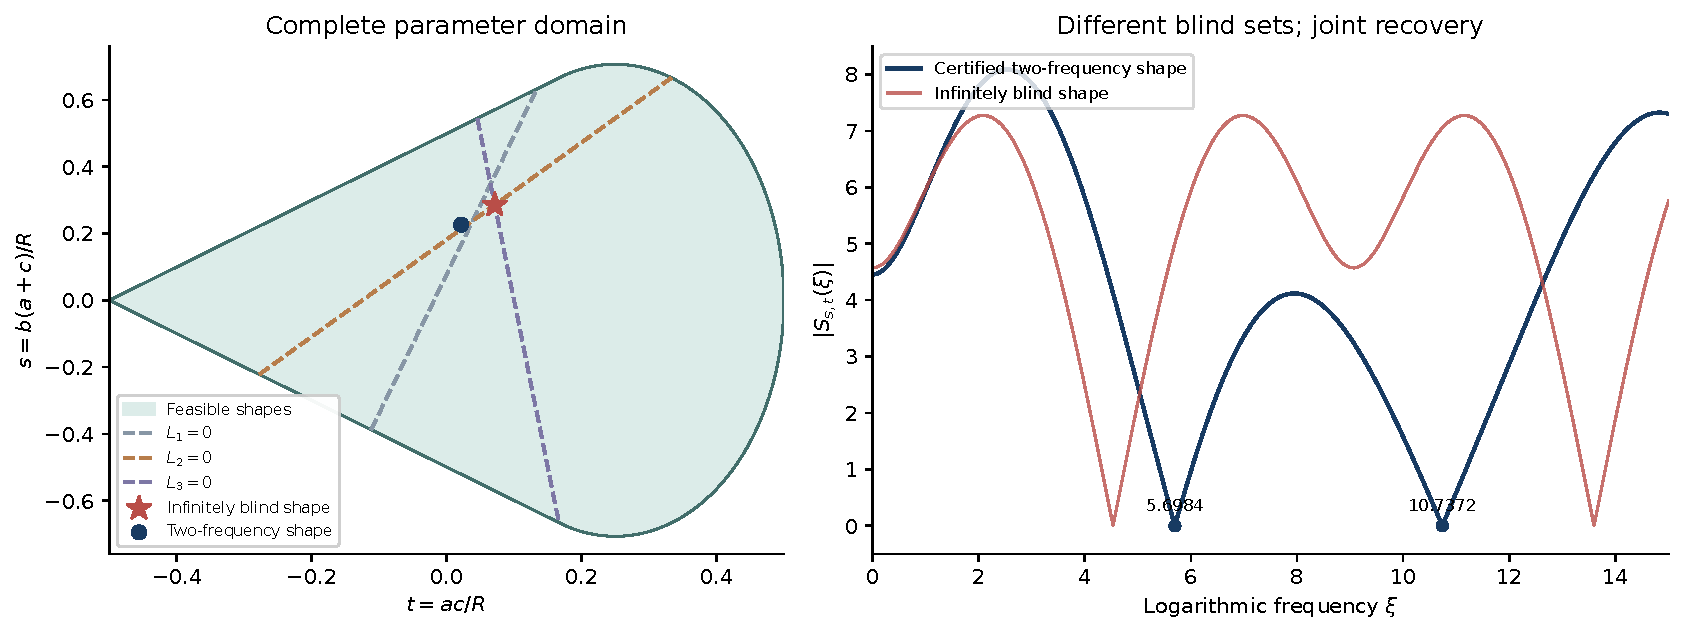
\includegraphics[width=\textwidth]{figures/five_shapes.pdf}
 \caption{Left: the complete shape domain and the three lines on which a pair
 can lose uniform finite-symbol separation. Right: the certified two-frequency
 shape and the unique infinitely blind shape have different blind sets.
 The curves are illustrations; the root existence proof is the exact certificate.}
 \label{fig:shapes}
\end{figure}

\begin{proposition}[Exceptional shapes are small]\label{prop:generic}
The feasible shapes with at least one blind real frequency form a set of
two-dimensional Lebesgue measure zero and a meagre subset of the parameter plane.
\end{proposition}
\begin{proof}
For fixed $\xi$, the real and imaginary parts of $S_{s,t}(\xi)=0$ are affine
linear equations in $(s,t)$. At any feasible solution their coefficient matrix
is nonsingular: if it were singular, a consistent affine system would contain
a whole line of real solutions. If $\Im z\ne0$, the elimination proof of
Theorem~\ref{thm:pair} rules out even two real solutions, without needing
feasibility. If $z=\pm1$ and $\xi\ne0$, in coordinates $(t,v)$ the coefficient
of $t$ is nonzero and real, whereas that of $v$ has imaginary part
$27\Im u\ne0$. At $\xi=0$ there is no feasible solution.
On each open interval where the determinant is nonzero, the unique solution
$(s(\xi),t(\xi))$ is real analytic. Cover these intervals by countably many
compact subintervals. Each analytic image has measure zero and empty interior,
and is compact, hence nowhere dense. The union contains every exceptional shape.
\end{proof}

\section{From symbols to positive spectral counts}

We now supply the analytic implication used to interpret the classification.
Let $A$ be a positive locally finite Borel measure on $[0,\infty)$ satisfying
\begin{equation}\label{eq:tailhyp}
 \int_1^\infty x^{-4}\dd A(x)<\infty.
\end{equation}
Write $A(T)=A([0,T])$, and define
\begin{align}\label{eq:variance}
 K_w(x)&=\frac{|P(e^{\ii x})|^2}{x^4},&
 U_w(h)&=h^4\int_0^\infty K_w(hx)\dd A(x),\\
 \B(w)&=\frac1\pi\int_0^\infty K_w(x)\dd x
 =\frac{R(4+2s)}6>0.&\notag
\end{align}
The kernel extends continuously at zero. If $A$ has an atom there, its contribution
is $O(h^4)$ and is irrelevant to the normalization $\tauh$.

\begin{theorem}[Two-variance recovery]\label{thm:recovery}
Let $w^{(1)},w^{(2)}$ be five-point contrasts with distinct shapes.
The following are equivalent:
\begin{enumerate}[label=\textup{(\alph*)}]
\item $\pi A(T)/(T\log T)\to d$ for a finite $d\ge0$;
\item both $U_{w^{(j)}}(h)/(\tauh)$ have finite limits as $h\downarrow0$;
\item both have finite limits along one sequence $h_n\downarrow0$ with $h_{n+1}/h_n\to1$.
\end{enumerate}
In either limiting formulation, the limits necessarily equal $d\B(w^{(j)})$.
For one contrast the analogous equivalence holds exactly when its blind set is empty.
\end{theorem}

\subsection{An injectivity lemma}

Put $\Phi(y)=\cos y-1+y^2/2$. The cancellations \eqref{eq:moments} give
\begin{equation}\label{eq:phi}
 |P(e^{\ii y})|^2=2\sum_{i<j}w_iw_j\Phi((j-i)y).
\end{equation}
Two integrations by parts and $\int_0^\infty(1-\cos y)y^{-2}\dd y=\pi/2$
give $\int_0^\infty\Phi(y)y^{-4}\dd y=\pi/12$, proving the formula for $\B$.

\begin{lemma}\label{lem:injective}
Let $\sigma$ be a signed measure on $(0,\infty)$ with total variation
$|\sigma|((0,X])\le C X$ for every $X>0$.
If
\[
 \int_0^\infty |P_j(e^{\ii ux})|^2x^{-4}\dd\sigma(x)=0
 \quad(u>0)
\]
for a finite family whose symbols have no common real zero, then $\sigma=0$.
\end{lemma}
\begin{proof}
Define $R_\sigma(u)=\int\Phi(ux)x^{-4}\dd\sigma(x)$ for real $u$.
The estimate $|\Phi(y)|\ll\min(|y|^4,|y|^2)$, split at $x=1/|u|$,
gives $R_\sigma(u)=O(|u|^3)$. It is continuous and even.
By \eqref{eq:phi}, $H(v)=e^{-3v}R_\sigma(e^v)$ is a bounded function
satisfying finite translation equations whose Fourier multipliers are
$\Sym_{w^{(j)}}(\xi)$. In the sense of tempered distributions,
$\Sym_{w^{(j)}}\widehat H=0$. For a compactly supported smooth test function,
divide it by the positive smooth function $\sum_j|\Sym_{w^{(j)}}|^2$ and
sum these equations after multiplication by the conjugate symbols.
It follows that $\widehat H=0$, hence $R_\sigma=0$.
In distributions,
\[
 R_\sigma^{(4)}(u)=\int_0^\infty\cos(ux)\dd\sigma(x).
\]
Testing against Schwartz functions justifies differentiating: near zero the
fourth derivative cancels $x^{-4}$, and at infinity rapid Fourier decay
controls the measure of linear growth. The right side is the Fourier transform
of the even extension of $\sigma$, giving half the mass to each reflection.
Fourier injectivity therefore gives $\sigma=0$.
\end{proof}

\subsection{Compactness and recovery}

\begin{proof}[Proof of Theorem~\ref{thm:recovery}]
For $T>2$ let $\mu_T(B)=\pi A(TB)/(T\log T)$.
A counting limit $d$ implies vague convergence $\mu_T\to d\dd x$ and
$A(T)=O((1+T)\log(2+T))$. On dyadic intervals beyond $X\ge1$ this growth gives
\[
 \int_X^\infty x^{-4}\dd\mu_T(x)
 \ll X^{-3}(1+\log(2X))
\]
uniformly for $T>2$. Since $K_w$ is bounded at zero and is $O(x^{-4})$
at infinity, convergence of its integral proves (a)$\Rightarrow$(b).
The implication (b)$\Rightarrow$(c) is immediate.

Conversely, bounded normalized measurements for just one nonzero contrast
already give $A(T)=O(T\log T)$. To see this, choose small $\delta>0$ such
that $P(e^{\ii x})$ has no zero on $[\delta/3,2\delta]$.
Choose a mesh point $h_n\sim\delta/T$. On $T/2\le x\le T$ the numerator
$|P(e^{\ii h_nx})|^2$ is bounded below, so the measurement bounds
$A([T/2,T])\ll T\log T$. Sum over dyadic intervals.
This works even when $P$ has a zero of order greater than two at $1$.

The measures $\mu_T$ are now relatively compact for vague convergence on
$[0,\infty)$, and each limit $\nu$ satisfies $\nu([0,X])\ll X$.
For every fixed $u>0$ choose mesh points with $Th_n\to u$.
Compact convergence of the kernels, their uniform tail bounds, and
$\log(1/h_n)/\log T\to1$ show that a tangent $\nu$ satisfies
\begin{equation}\label{eq:tangent-measurement}
 \frac1\pi\int_0^\infty|P_j(e^{\ii ux})|^2x^{-4}\dd\nu(x)
 =u^3\ell_j,
\end{equation}
where $\ell_j$ is the corresponding measured limit.

The normalized dilation $\nu_v(B)=\nu(vB)/v$ is also a tangent:
replace a convergent sequence $T_k$ by $vT_k$ and use
$\log(vT_k)/\log T_k\to1$.
Equation \eqref{eq:tangent-measurement} holds with the same $\ell_j$
for $\nu_v$. Apply Lemma~\ref{lem:injective} to $\nu_v-\nu$;
Theorem~\ref{thm:pair} supplies its hypothesis. Thus $\nu_v=\nu$ for
every $v>0$. A locally finite positive measure on the half-line with this
homogeneity is $d\dd x$: its cumulative function equals $dX$.
Equation \eqref{eq:tangent-measurement} gives $\ell_j=d\B(w^{(j)})$,
so $d$ is independent of the chosen tangent. Every tangent is the same,
and evaluation on $[0,1]$ proves (a).

The same proof works for a single zero-free symbol. If it has a blind
frequency $\omega\ne0$, take on $x\ge1$
\begin{equation}\label{eq:counterdensity}
 \dd A(x)=\frac{\log x}{\pi}\bigl(1+\epsilon\cos(\omega\log x)\bigr)\dd x,
 \qquad 0<\epsilon<1.
\end{equation}
Substitution in \eqref{eq:phi} yields the absolutely convergent identity
\begin{equation}\label{eq:mellin}
 \int_0^\infty K_w(y)y^{\ii\xi}\dd y
 =2\Sym_w(-\xi)\int_0^\infty\Phi(y)y^{-4+\ii\xi}\dd y.
\end{equation}
The oscillatory coefficient vanishes at $\omega$, so the variance limit
is $\B(w)$. Yet
$\pi A(T)/(T\log T)=1+\epsilon\Re(T^{\ii\omega}/(1+\ii\omega))+o(1)$
does not converge. The integrable $K_w(y)|\log y|$ controls the error terms.
\end{proof}

\section{Exactly what a single defective variance leaves unknown}

\begin{theorem}[All positive tangent measures]\label{thm:tangents}
Suppose $U_w(h)/(\tauh)\to d\B(w)$, either continuously or on a mesh
as in Theorem~\ref{thm:recovery}. Then all tangent measures of
$\mu_T=\pi A(T\,\cdot)/(T\log T)$ are as follows.
\begin{enumerate}[label=\textup{(\roman*)}]
\item If the positive blind frequencies are $\omega_1,\ldots,\omega_k$,
$k\le2$, each tangent has density
\begin{equation}\label{eq:finite-tangent}
 d+\Re\sum_{j=1}^k c_jx^{\ii\omega_j}\quad(x>0),
\end{equation}
where this density is nonnegative everywhere. For $k=0$ it is simply $d$.
\item At the unique shape \eqref{eq:infinite}, every tangent has density
\begin{equation}\label{eq:infinite-tangent}
 d+f(\log x),\qquad
 f(v+\log2)=-f(v)\text{ a.e.},\qquad |f(v)|\le d\text{ a.e.}
\end{equation}
\end{enumerate}
Conversely, every profile described in (i) or (ii) occurs as a tangent for
some positive $A$ with this variance limit. These converse examples are
abstract spectra, not claimed to be the zero spectrum of an Euler product.
\end{theorem}
\begin{proof}
The compactness argument above applies, and for $\sigma=\nu-d\dd x$
the function $H$ in Lemma~\ref{lem:injective} is bounded with Fourier
transform supported on the blind set.
For a finite blind set a distribution with this support is a finite sum
of derivatives of point masses; hence $H$ is a finite sum of exponentials
times polynomials. Boundedness makes every polynomial constant. Indeed,
if the largest degree were positive, dividing by that power of $v$ as
$v\to+\infty$ would make a nonzero finite trigonometric sum tend to zero,
contrary to its strictly positive limiting mean square.
Reality pairs conjugate frequencies.

The map from $\Re(c x^{\ii\omega})\dd x$ to $H$ is a nonzero scalar
multiple of $\Re(c e^{-\ii\omega v})$: substitution gives the scalar
$J(\omega)=\int_0^\infty\Phi(y)y^{-4+\ii\omega}\dd y$.
This scalar cannot be zero, since otherwise the injective map
$\sigma\mapsto R_\sigma$ in the final Fourier-injectivity step of
Lemma~\ref{lem:injective} would send a
nonzero oscillatory measure to zero. Thus these densities realize every
possible finite-frequency $H$; injectivity gives \eqref{eq:finite-tangent}.
Positivity of $\nu$ imposes the stated nonnegativity.

For the infinite shape, put $L=\log2$ and let $T_L$ translate functions
by $L$. Equation \eqref{eq:specialfactor} gives
$(T_L+1)(2T_L-1)H=0$. The bounded function $G=(T_L+1)H$
satisfies $G(v+L)=G(v)/2$, and iteration towards $-\infty$ gives $G=0$.
Hence $H(v+L)=-H(v)$, or $R_\sigma(2u)=-8R_\sigma(u)$.
The measure $\sigma_2(B)=\sigma(2B)/2$ has
$R_{\sigma_2}(u)=8R_\sigma(u/2)=-R_\sigma(u)$.
Injectivity gives
\begin{equation}\label{eq:anti-measure}
 \sigma(2B)=-2\sigma(B).
\end{equation}
On a bounded Lebesgue-null set $B$, both $\sigma(B)=\nu(B)$ and
$\sigma(2B)=\nu(2B)$ are nonnegative, so both vanish.
Thus $\sigma$ is absolutely continuous. Its density $g$ satisfies
$g(2x)=-g(x)$ almost everywhere. Positivity and this sign reversal give
$-d\le g\le d$. Setting $f(v)=g(e^v)$ proves (ii).

For the converse, set $\dd A(x)=\pi^{-1}\log x\,[d+g(x)]\dd x$
on $x\ge1$, with $g$ any allowed profile minus $d$.
In the finite case \eqref{eq:mellin} kills each oscillation.
There are arbitrarily large $T$ with all phases $T^{\ii\omega_j}$
arbitrarily close to $1$, by recurrence of rotations on a compact torus;
along such a sequence the desired tangent occurs.
In the infinite case the normalized response satisfies
\begin{equation}\label{eq:kernel-special}
 K_w(y)/R=\tfrac47K_0(y)+\tfrac87K_0(2y),
 \qquad K_0(y)=|1-e^{\ii y}|^4/y^4.
\end{equation}
For every $v$, the integral of this kernel against $f(\log y+v)$
vanishes by substitution and anti-periodicity. The residual logarithmic
term is $O(1/\log(1/h))$ after normalization, because
$K_w(y)|\log y|$ is integrable. Taking $T=4^n$ gives the desired tangent.
\end{proof}

\begin{corollary}[Removing the hidden oscillations by finitely many dilations]
Let $a(T)=\pi A(T)/(T\log T)$ under the preceding hypotheses.
For a finite blind set put $L_j=\exp(\pi/\omega_j)$. Then
\begin{equation}\label{eq:repair-average}
 \frac1{2^k}\sum_{E\subseteq\{1,\ldots,k\}}
 a\left(T\prod_{j\in E}L_j\right)\longrightarrow d.
\end{equation}
Thus at most four dilations suffice. For the infinitely blind shape,
$[a(T)+a(2T)]/2\to d$.
\end{corollary}
\begin{proof}
On any tangent subsequence, evaluation on $[0,u]$ is continuous because
the tangents in Theorem~\ref{thm:tangents} have densities. A finite mode
contributes $\Re(c_j u^{\ii\omega_j}/(1+\ii\omega_j))$ to the limit of
$a(uT)$. The factor $(1+L_j^{\ii\omega_j})/2=0$ kills it in
\eqref{eq:repair-average}. For (ii), \eqref{eq:anti-measure} gives the
two-term identity directly. Relative compactness promotes these
subsequential identities to the asserted limits.
\end{proof}

\section{The consequence for prime fluctuations and zeta zeros}

Assume RH, as provided by the upstream input. For $x>1$ put
\[
 S(x)=\sum_{n\le x}\Lambda(n)\left(\frac1n-\frac1x\right),\qquad
 E(v)=e^{v/2}\bigl(S(e^v)-v+\gamma_E+1\bigr).
\]
If $\gamma>0$ runs over distinct positive ordinates of nontrivial zeta
zeros and $m_\gamma$ denotes multiplicity, the smoothed explicit formula is
\begin{equation}\label{eq:explicit}
 E(v)=2\sum_{\gamma>0}\frac{m_\gamma\cos(\gamma v)}{1/4+\gamma^2}
 +O((1+v)e^{-v/2}).
\end{equation}
This is the source article's \texttt{zer:lem:ramp} and
\texttt{zer:sec:coalesce} \cite{ProveIt}. One derivation integrates
$-\zeta'/\zeta(1+z)e^{vz}/[z(z+1)]$: the double pole at zero gives
$v-\gamma_E-1$, and a zero $\rho$ gives
$e^{(\rho-1)v}/[\rho(1-\rho)]$. Trivial zeros and the pole at $z=-1$
give the stated smaller terms. The usual zero count gives absolute
convergence of the zero series under RH.

For a contrast $w$ let its long-time variance be
\begin{equation}\label{eq:primevariance}
 V_w(h)=\lim_{X\to\infty}\frac1X\int_0^X
 \left|\sum_{j=0}^4w_j E(v+jh)\right|^2\dd v.
\end{equation}
Absolute convergence in \eqref{eq:explicit} permits termwise long-time
averaging. Distinct frequencies are orthogonal under this averaging,
without any independence hypothesis. Thus
\begin{equation}\label{eq:spectralvariance}
 V_w(h)=2\sum_{\gamma>0}
 \frac{m_\gamma^2|P(e^{\ii h\gamma})|^2}{(1/4+\gamma^2)^2}.
\end{equation}
Take $A=2\sum_{\gamma>0}m_\gamma^2\delta_\gamma$ and
$M_2(T)=\sum_{0<\gamma\le T}m_\gamma^2$.
The elementary bounds $m_\gamma=O(\log(2+\gamma))$ and
$N(T)=O(T\log(2+T))$ imply $M_2(T)=O(T\log^2(2+T))$ and
$\int(1+x^2)^{-1}\dd A(x)<\infty$.
Using $|P(e^{\ii hx})|^2\ll h^4x^4$ gives
\[
 |V_w(h)-U_w(h)|
 \ll h^4\int_0^\infty\frac{\dd A(x)}{1+x^2}=O(h^4)
 =o(\tauh).
\]
There is no central zeta zero; for example the alternating eta series
is positive at $1/2$ whereas $1-2^{1-1/2}\ne0$.

\begin{corollary}[Five prime scales determine the multiplicity limit]\label{cor:zeta}
Choose any two five-point contrasts with distinct shapes. Then
\[
 \kappa(T):=\frac{2\pi M_2(T)}{T\log T}
\]
has a finite limit if and only if both $V_{w^{(j)}}(h)/(\tauh)$ have
finite limits, even if they are measured only on $h_n\downarrow0$ with
$h_{n+1}/h_n\to1$. When the limit is $\kappa$, the two variance limits
are $\kappa\B(w^{(j)})$. For one contrast, the analytic classification
and tangent descriptions above apply to its possible failure of recovery.
\end{corollary}

This theorem concerns whether and how a limit can be recovered. It does not
assert that $\kappa(T)$ converges, or that the actual zeta zeros realize one
of the abstract oscillatory examples. Those are separate arithmetic questions.
The two measured contrasts use the same five positions $v,v+h,\ldots,v+4h$.
No additional prime scales are needed to remove the single-contrast ambiguity.

\section{Reproducibility and remaining questions}

The archive includes the complete source and compiled PDF of this paper,
the rational existence checker and its output, exact symbolic checks of the
response and symbol identities, a shape-domain figure, and a source/novelty
record. The sharpness checker has no third-party dependencies. Symbolic
verification uses SymPy, and figure generation uses NumPy and Matplotlib.
Neither a numerical search nor a plotting routine is used in a proof except
through the explicitly described exact certificate.

The arguments identify every possible real blind frequency, but the phase
condition for arbitrary real coefficients is inherently an exact equality.
A practical decision procedure with specified finite input encoding is a
different problem. Likewise the uniform gap in Theorem~\ref{thm:gap} is a
finite-symbol statement; an effective error bound for noisy, finite-height
measurements would have to track the analytic Mellin factor and tail estimates.
For six or more observations additional independent prime logarithms enter,
so the quadratic reduction and universal two-shape argument need not persist.

\begin{thebibliography}{9}
\raggedright
\bibitem{ProveIt}
V. Reshetnikov, \emph{ProveIt: Analysis/GeneralizedRiemannHypothesis},
commit \texttt{3413bfb1edb3636437f9cec7e5dd975869f7d120}, inspected 27 November 2026.
\href{https://github.com/VladimirReshetnikov/ProveIt/blob/3413bfb1edb3636437f9cec7e5dd975869f7d120/Analysis/GeneralizedRiemannHypothesis/Article/sections/zer.tex}{Pinned zero-statistics section};
\href{https://github.com/VladimirReshetnikov/ProveIt/blob/3413bfb1edb3636437f9cec7e5dd975869f7d120/Analysis/GeneralizedRiemannHypothesis/Article/README.md}{article status and inventory}.
\bibitem{FiveNodePrior}
ProveIt research report, \emph{The missing frequencies of five-point prime variances},
27 November 2026, Theorems 1 and 2. File \texttt{five\_node\_filters/five\_node\_frequencies.tex}
inside the incoming archive \texttt{dirichlet-coupled-zeros-and-prime-variances.zip},
at the same pinned revision.
\href{https://github.com/VladimirReshetnikov/ProveIt/blob/3413bfb1edb3636437f9cec7e5dd975869f7d120/Analysis/GeneralizedRiemannHypothesis/docs/incoming/dirichlet-coupled-zeros-and-prime-variances.zip}{Pinned incoming report}.
\bibitem{Wiener}
N. Wiener, Tauberian theorems, \emph{Annals of Mathematics} (2) \textbf{33}
(1932), 1--100. \href{https://doi.org/10.2307/1968102}{doi:10.2307/1968102}.
\bibitem{BinghamInoue}
N. H. Bingham and A. Inoue, \emph{Tauberian and Mercerian theorems for systems of kernels},
author-hosted paper. \url{https://home.hiroshima-u.ac.jp/inoue100/systems.pdf}.
\bibitem{Sutherland}
A. Sutherland, \emph{Verification files for the shorter Lean proof of RH and of GRH
for Dirichlet L-functions}, updated 27 November 2026, 17:27 UTC.
\url{https://math.mit.edu/~drew/shortgrh/}.
\end{thebibliography}
\end{document}
